 \documentclass[11pt]{beamer}
\usetheme{Warsaw}
\usepackage[utf8]{inputenc}
\usepackage{amsmath}
\usepackage{amsfonts}
\usepackage{amssymb}
\usepackage{tikz}
\usetikzlibrary{arrows,automata}
%\usepackage[latin1]{inputenc}

\author{Team Expeditus}
\title{UAV Autonomous Landing}
%\setbeamercovered{transparent} 
%\setbeamertemplate{navigation symbols}{} 
%\logo{} 
\institute{Dept. of Computer Science, SDSMT} 
%\date{} 
%\subject{} 
\begin{document}

\begin{frame}
\titlepage
\end{frame}

%\begin{frame}
%\tableofcontents
%\end{frame}

\begin{frame}{Introduction}
\textbf{UAV Autonomous Landing Project}\\
\vspace{12mm}
\textbf{Team Expeditus}\\
Jonathan Dixon, Dylan Geyer, Christopher Smith, Steven Huerta\\ 
\vspace{6mm}
\textbf{Sponsor}\\
Dr. Larry Pyeatt\\
\end{frame}

\begin{frame}{Goal}
\textbf{Goal}\\
\begin{itemize}
\item receive a set of waypoints
\item autonomously take-off
\item navigate through waypoints
\item return to launch pad
\item land on the pad with the correct orientation
\end{itemize}
\vspace{6mm}
\textbf{Limitations}\\
\begin{itemize}
\item landing platform is a fixed position
\item landing platform is a stable, horizontal surface
\item environment is ideal(no wind, gps available, no obstacles)
\end{itemize}

\end{frame}

\begin{frame}{Phase Objectives}
\textbf{Phase I}
\begin{itemize}
\item Build UAV 
\item Flight Controller Operating Correctly
\item Simulation Environment Available
\end{itemize}
\vspace{5mm}
\textbf{Phase II}
\begin{itemize}
\item Autonomous landing ready for simulation
\item Autonomous landing ready for UAV
\end{itemize}
\end{frame}

\begin{frame}{Testing}
\textbf{Phase I}
\begin{itemize}
\item Test manual flight of UAV
\item Test of flight controller autonomy on a course 
\end{itemize}
\vspace{5mm}
\textbf{Phase II}
\begin{itemize}
\item Test of simulated landing
\item Test of UAV autonomous landing on landing pad
\item Test of UAV task integration
\end{itemize}
\end{frame}

\begin{frame}{Approach - UAV}

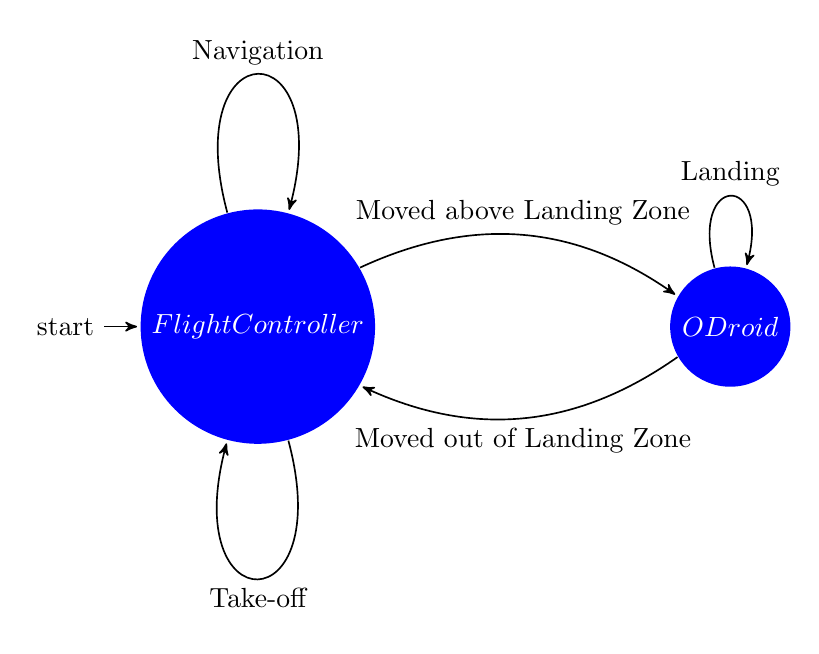
\begin{tikzpicture}[->,>=stealth',shorten >=1pt,auto,node distance=6cm,
                    semithick]
  \tikzstyle{every state}=[fill=blue,draw=none,text=white]

  \node[initial,state] (A)              {$Flight Controller$};
  \node[state]         (B) [right of=A] {$ODroid$};

  \path (A) edge [loop below] node {Take-off} (A)
            edge [loop above]  node {Navigation} (A)
            edge [anchor=center,bend left,above] node {Moved above Landing Zone} (B)
        (B) edge [loop above] node {Landing} (B)
            edge [anchor=center,bend left,left,below]  node {Moved out of Landing Zone} (A);
\end{tikzpicture}
\end{frame}

\begin{frame}{Approach - Software}
\begin{figure}
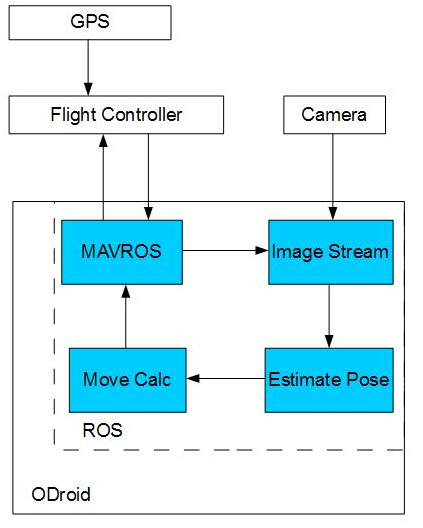
\includegraphics[width=.5\textwidth]{broad_approach1}
\end{figure}
\end{frame}

\begin{frame}{Approach - Landing Vision}
\begin{itemize}
	\item AR/QR tags for orientation and range.
	\item Colored blobs or LEDs for orientation.
	\item Example of AR Tag and colored circles similar
	\centerline{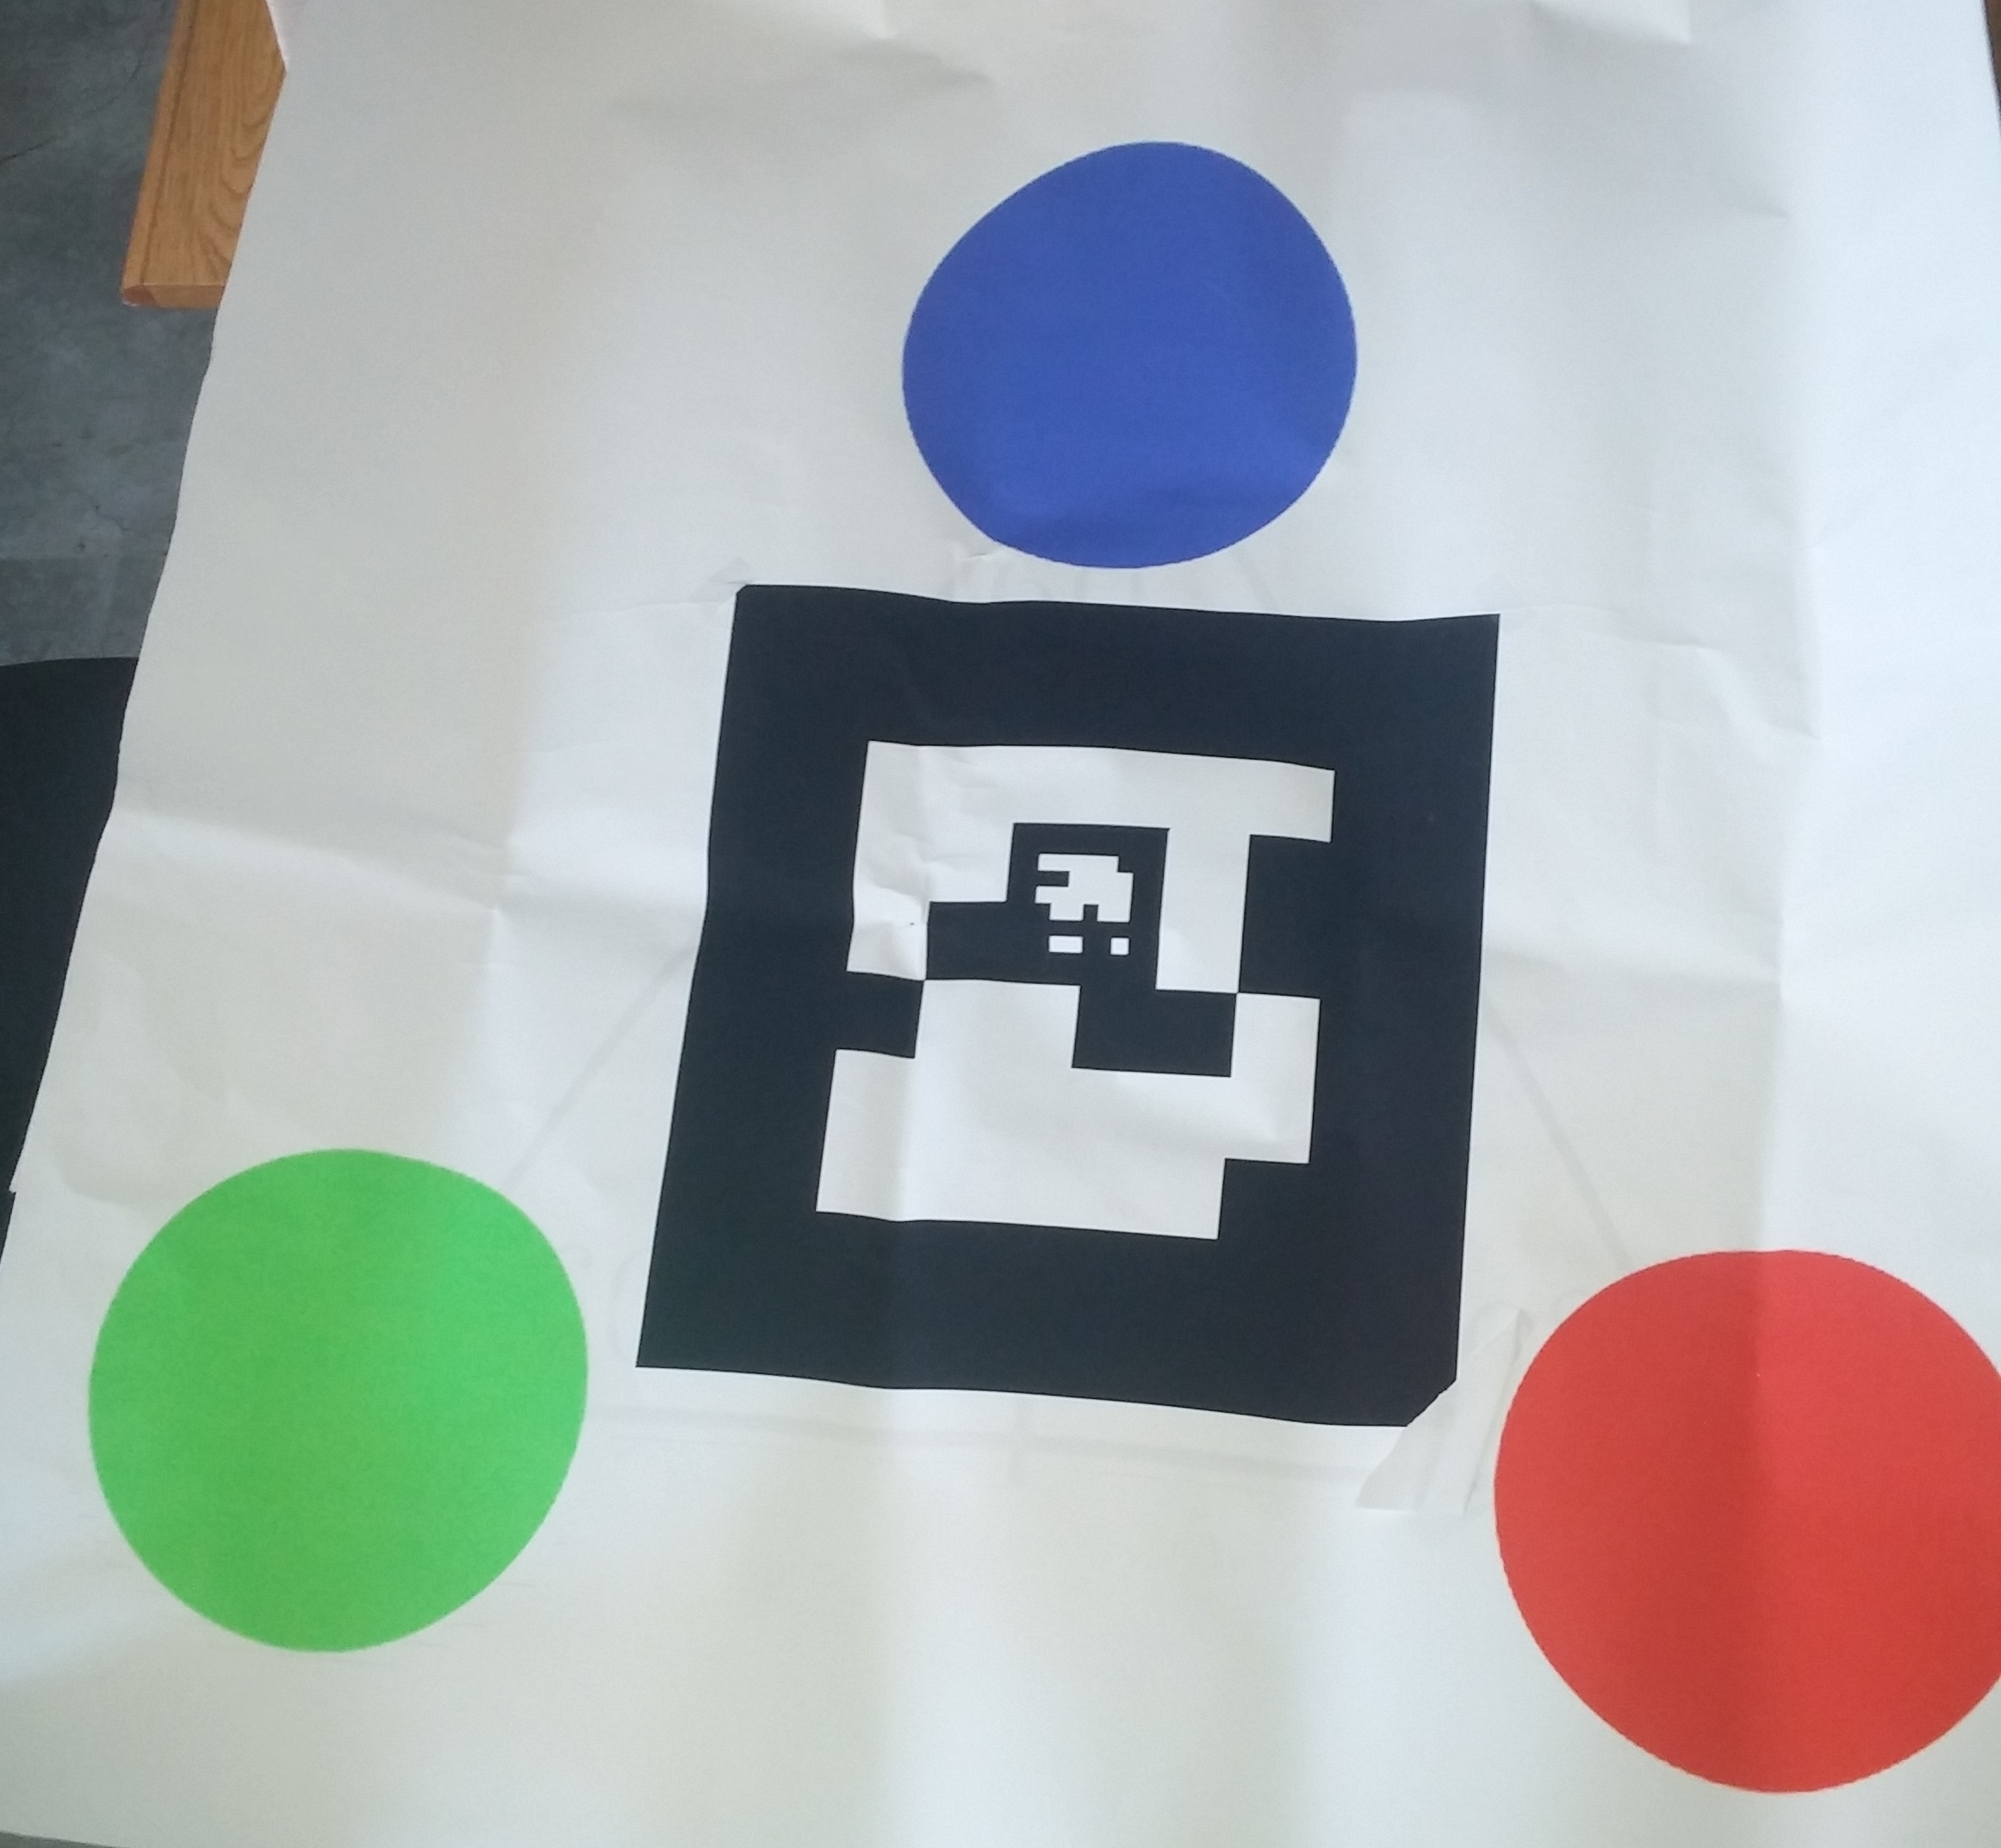
\includegraphics[scale=0.07]{images/example_pad_target.jpg}}
\end{itemize}
\end{frame}

\begin{frame}{Approach - Landing AI}
\textbf{Artificial Neural Network (ANN) Approach}:
\begin{itemize}
\item Use Flight Controller to reach landing pad waypoint
\item Switch to landing mode using ANN
\item Land on landing pad or get within some distance to switch to vision
\end{itemize}
\end{frame}


\begin{frame}{Development - Software}
\textbf{Development OS}: Ubuntu 14.04\\
\textbf{Languages}: C++ and Python\\
\vspace{5mm}
\textbf{Software Tools}
\begin{itemize}
\item Robot Operating System(ROS)
\item Gazebo
\item APM Planner
\end{itemize}
\end{frame}


\begin{frame}{Development - Software Contd.}
\textbf{Simulation \& Testing}: 
\begin{itemize}
\item Rotors Sim package - Provides Models for Gazebo
\end{itemize}
\centerline{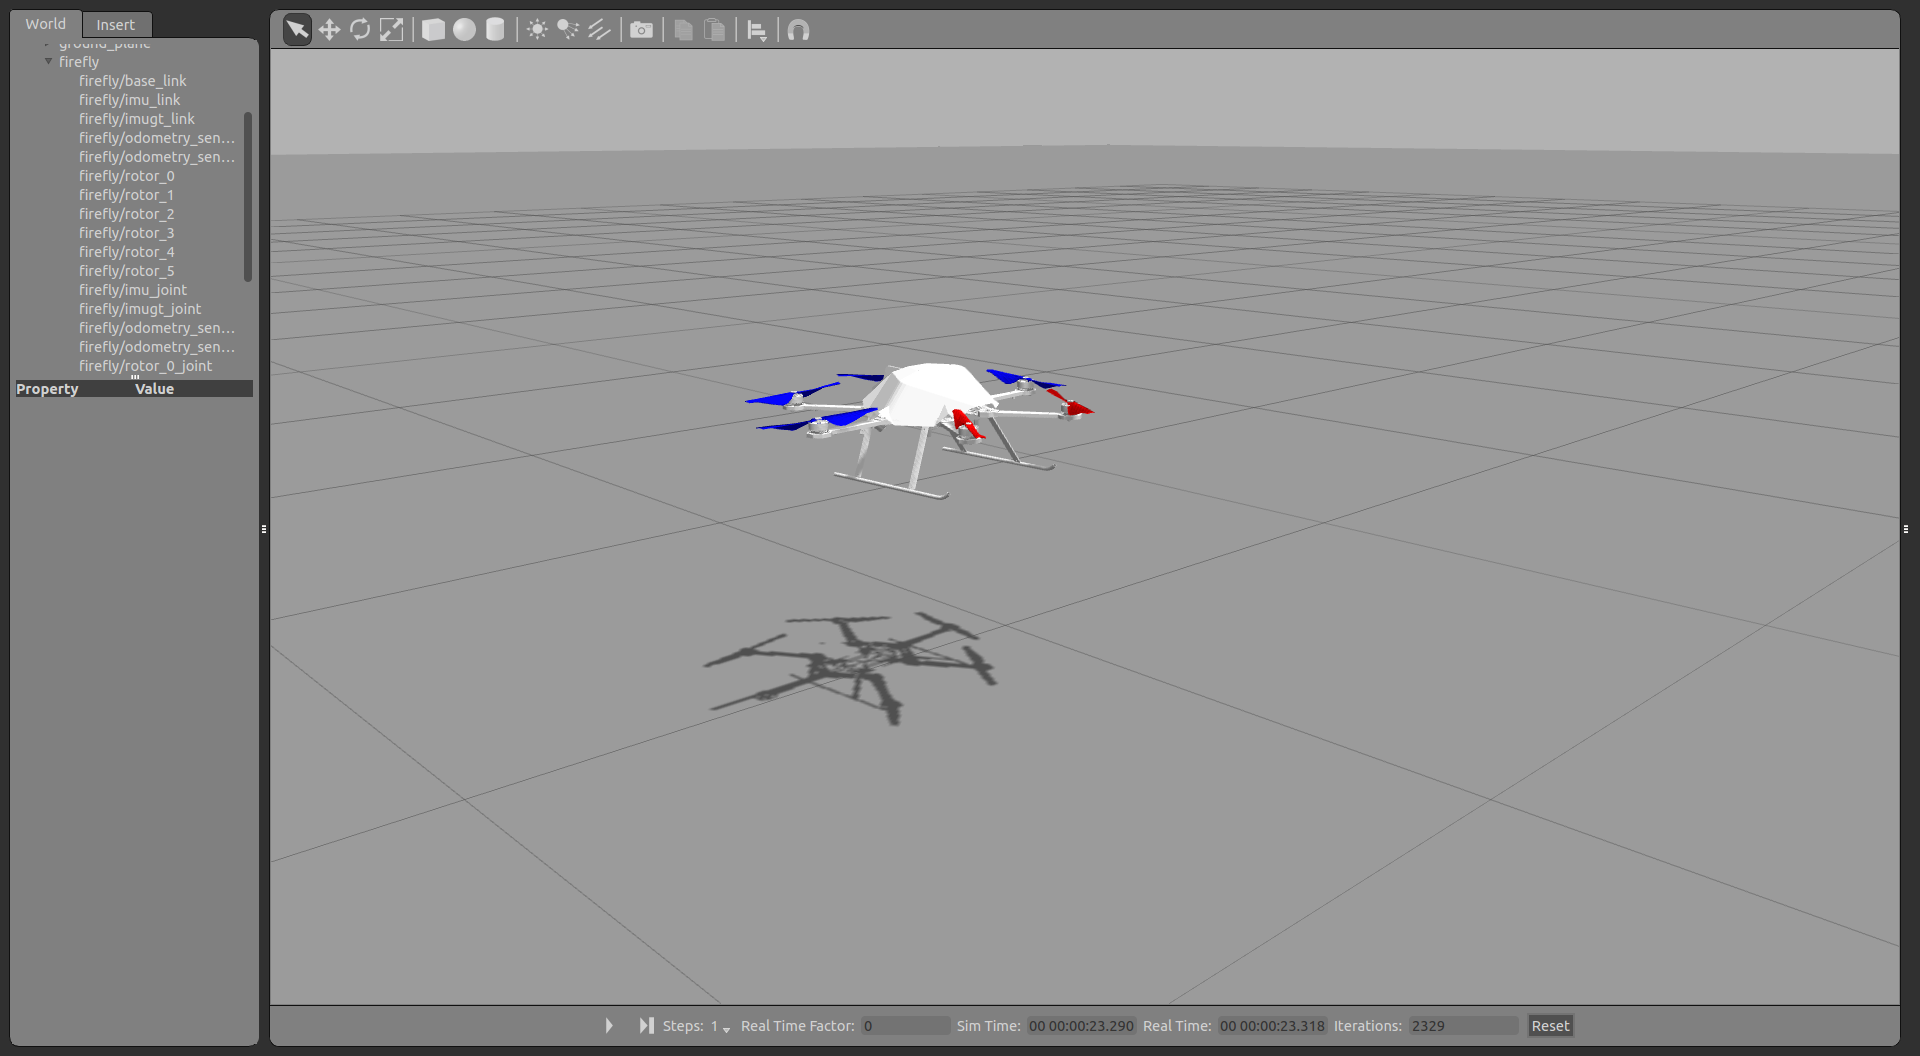
\includegraphics[scale=0.15]{images/Gazebo_Joy.png}}
\end{frame}

\begin{frame}{Development - Software Contd.}
\begin{itemize} 
\item MavRos - Communication with Pixhawk through ROS
\item Testing - All components will be tested in simulation before being deployed on UAV
\end{itemize}
\centerline{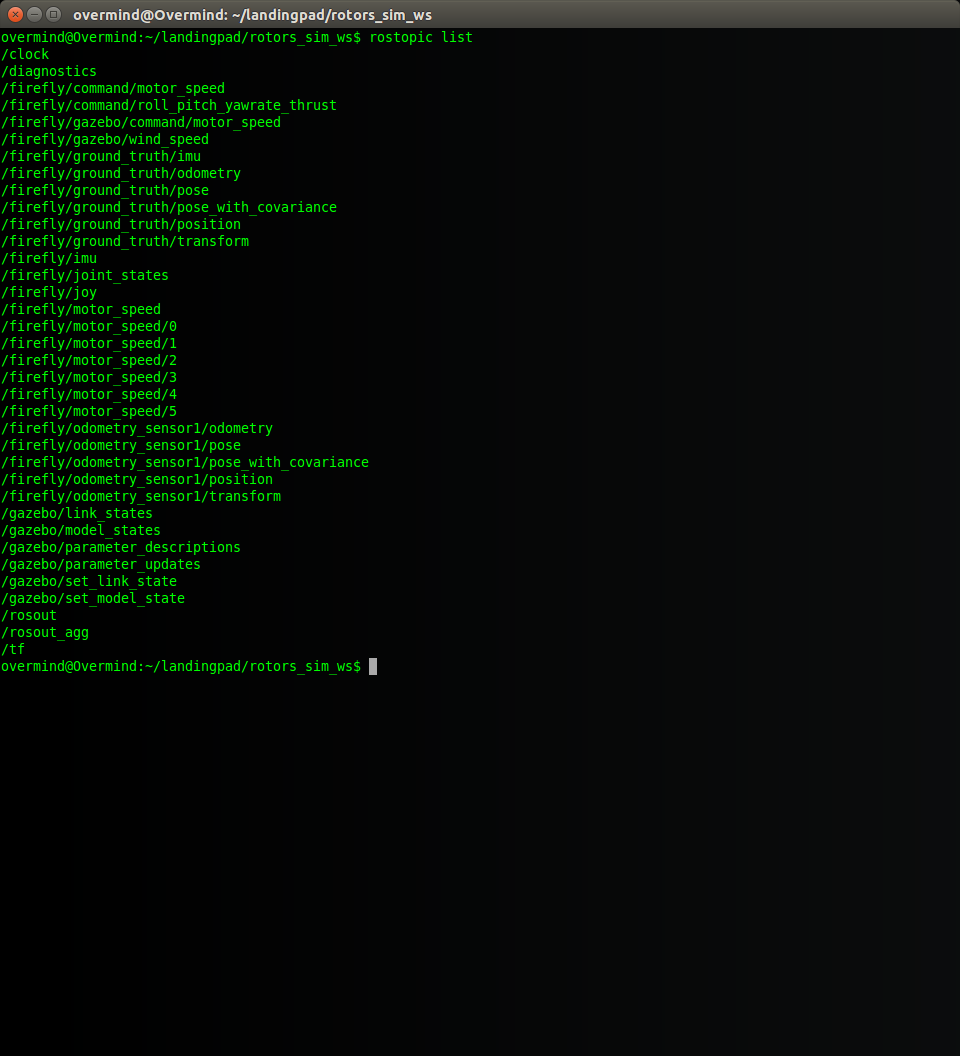
\includegraphics[scale=0.15]{images/Ros_Topics.png}}
\end{frame}

\begin{frame}{Development - Hardware}

	\begin{tabular}[c]{| c | c | c |}
		\hline
		Item & Quantity & Total Weight\\
		\hline
		DC Motor & 6 & 372g\\
		\hline
		Frame & 1 & 1300g\\
		\hline
		Battery & 1 & 680g\\
		\hline
		Camera & 2 & 140g\\
		\hline
		ODroid & 1 & 48g\\
		\hline
		GPS Module & 1 & 17g\\
		\hline
		\multicolumn{2}{| r |}{\textbf{Total}} & 2557g\\
		\hline
	\end{tabular}
	\hfill \break \\
	6 Motors at 100\% produces 5820g of lift\\

	Motors must run at 2557g / 5820g = 44\%
\end{frame}

\begin{frame}{Development - Hardware Continued...}
	\textbf{Hardware Constraints}
	\begin{itemize}
		\item 6000mAh Battery
		\item Power ODroid + Peripherals
		\item Power 6x DC Motors
	\end{itemize}
	
	\centerline{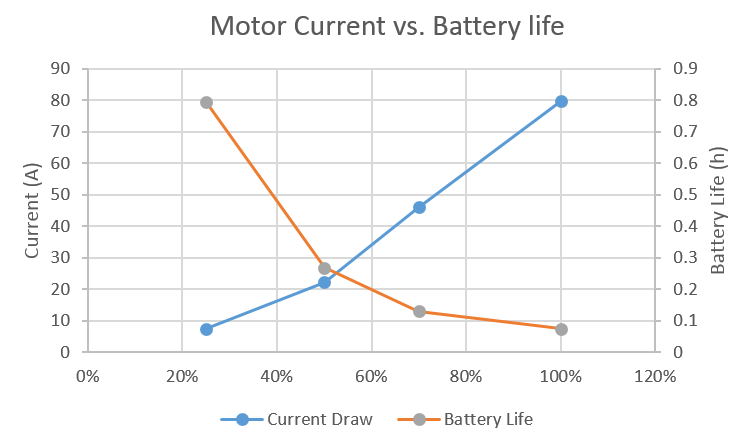
\includegraphics[width=0.75\textwidth]{Power_BatteryLife}}
	
\end{frame}

\begin{frame}{Development - Hardware Continued...}
	\textbf{Computational Constraints}
	\begin{itemize}
		\item Images: 976 x 582 pixels at $\ge$ 30 images/sec
		\item Real time image processing requires $30 * 976 * 582 = 17M  flops$
		\item ODroid has 8 cores at 1.4 GHz
		\begin{itemize}
			\item Ideal throughput $\sim$1 Billion operations/sec
		\end{itemize}
	\end{itemize}
\end{frame}

\begin{frame}{Cost}
\centering{
\begin{tabular}[c]{| l | r | l | r |}
\hline
\multicolumn{2}{| c |}{\textbf{Build 1}} & \multicolumn{2}{| c |}{\textbf{Build 2}} \\
\hline
Item & Cost & Item & Cost \\
\hline
Controller & \$199.99 & Controller & \$199.99\\
\hline
ODroid 	   & \$75.95  & ODroid 	   & \$75.95 \\
\hline
Sensors    & \$167.23 & Sensors    & \$167.23 \\
\hline
Frame Kit  & \$242.48 &  &\\
\hline
Power Kit  & \$119.98 &  &\\
\hline
Radio Set  & \$100.00 &  &\\
\hline
Extra Parts & \$95.15 &  &\\
\hline
\textbf{TOTAL} & \$1000.78 & \textbf{TOTAL} & \$443.17\\
\hline
\end{tabular}
}
\end{frame}

\begin{frame}{Work Accomplished}
\textbf{General}
\begin{itemize}
\item Review previous iteration documentation \& code
\item Begin pilot training for manual control
\item Review Landing Pad model with Landing Pad teams
\end{itemize}
\vspace{4mm}
\textbf{Setup Development Environment}
\begin{itemize}
\item Ubuntu 14.04
\item Gazebo/Rviz
\item ROS - Jade Distro
\end{itemize}
\vspace{4mm}
\textbf{Inspect Current Quadrotor}
\begin{itemize}
\item Identify missing or non-functioning components 
\item Generate order list
\end{itemize}
\end{frame}

\begin{frame}{Setbacks/Risk}
\textbf{Risk}
\begin{itemize}
\item Reliance on Flight Controller
\item Dependency on external team for Landing Pad
\item No UAV Backup
\end{itemize}
\vspace{6mm}
\textbf{Setbacks}
\begin{itemize}
\item Non-functional components
\item Little carry-over from previous year
\end{itemize}
\end{frame}

\begin{frame}[t]{Conclusion}
\textbf{Team Expeditus}
\begin{itemize}
\item has adapted focus of tasks based on conditions
\item is making progress on those tasks
\item is on track to complete Phase I goals
\end{itemize}

\begin{figure}
    \centering
    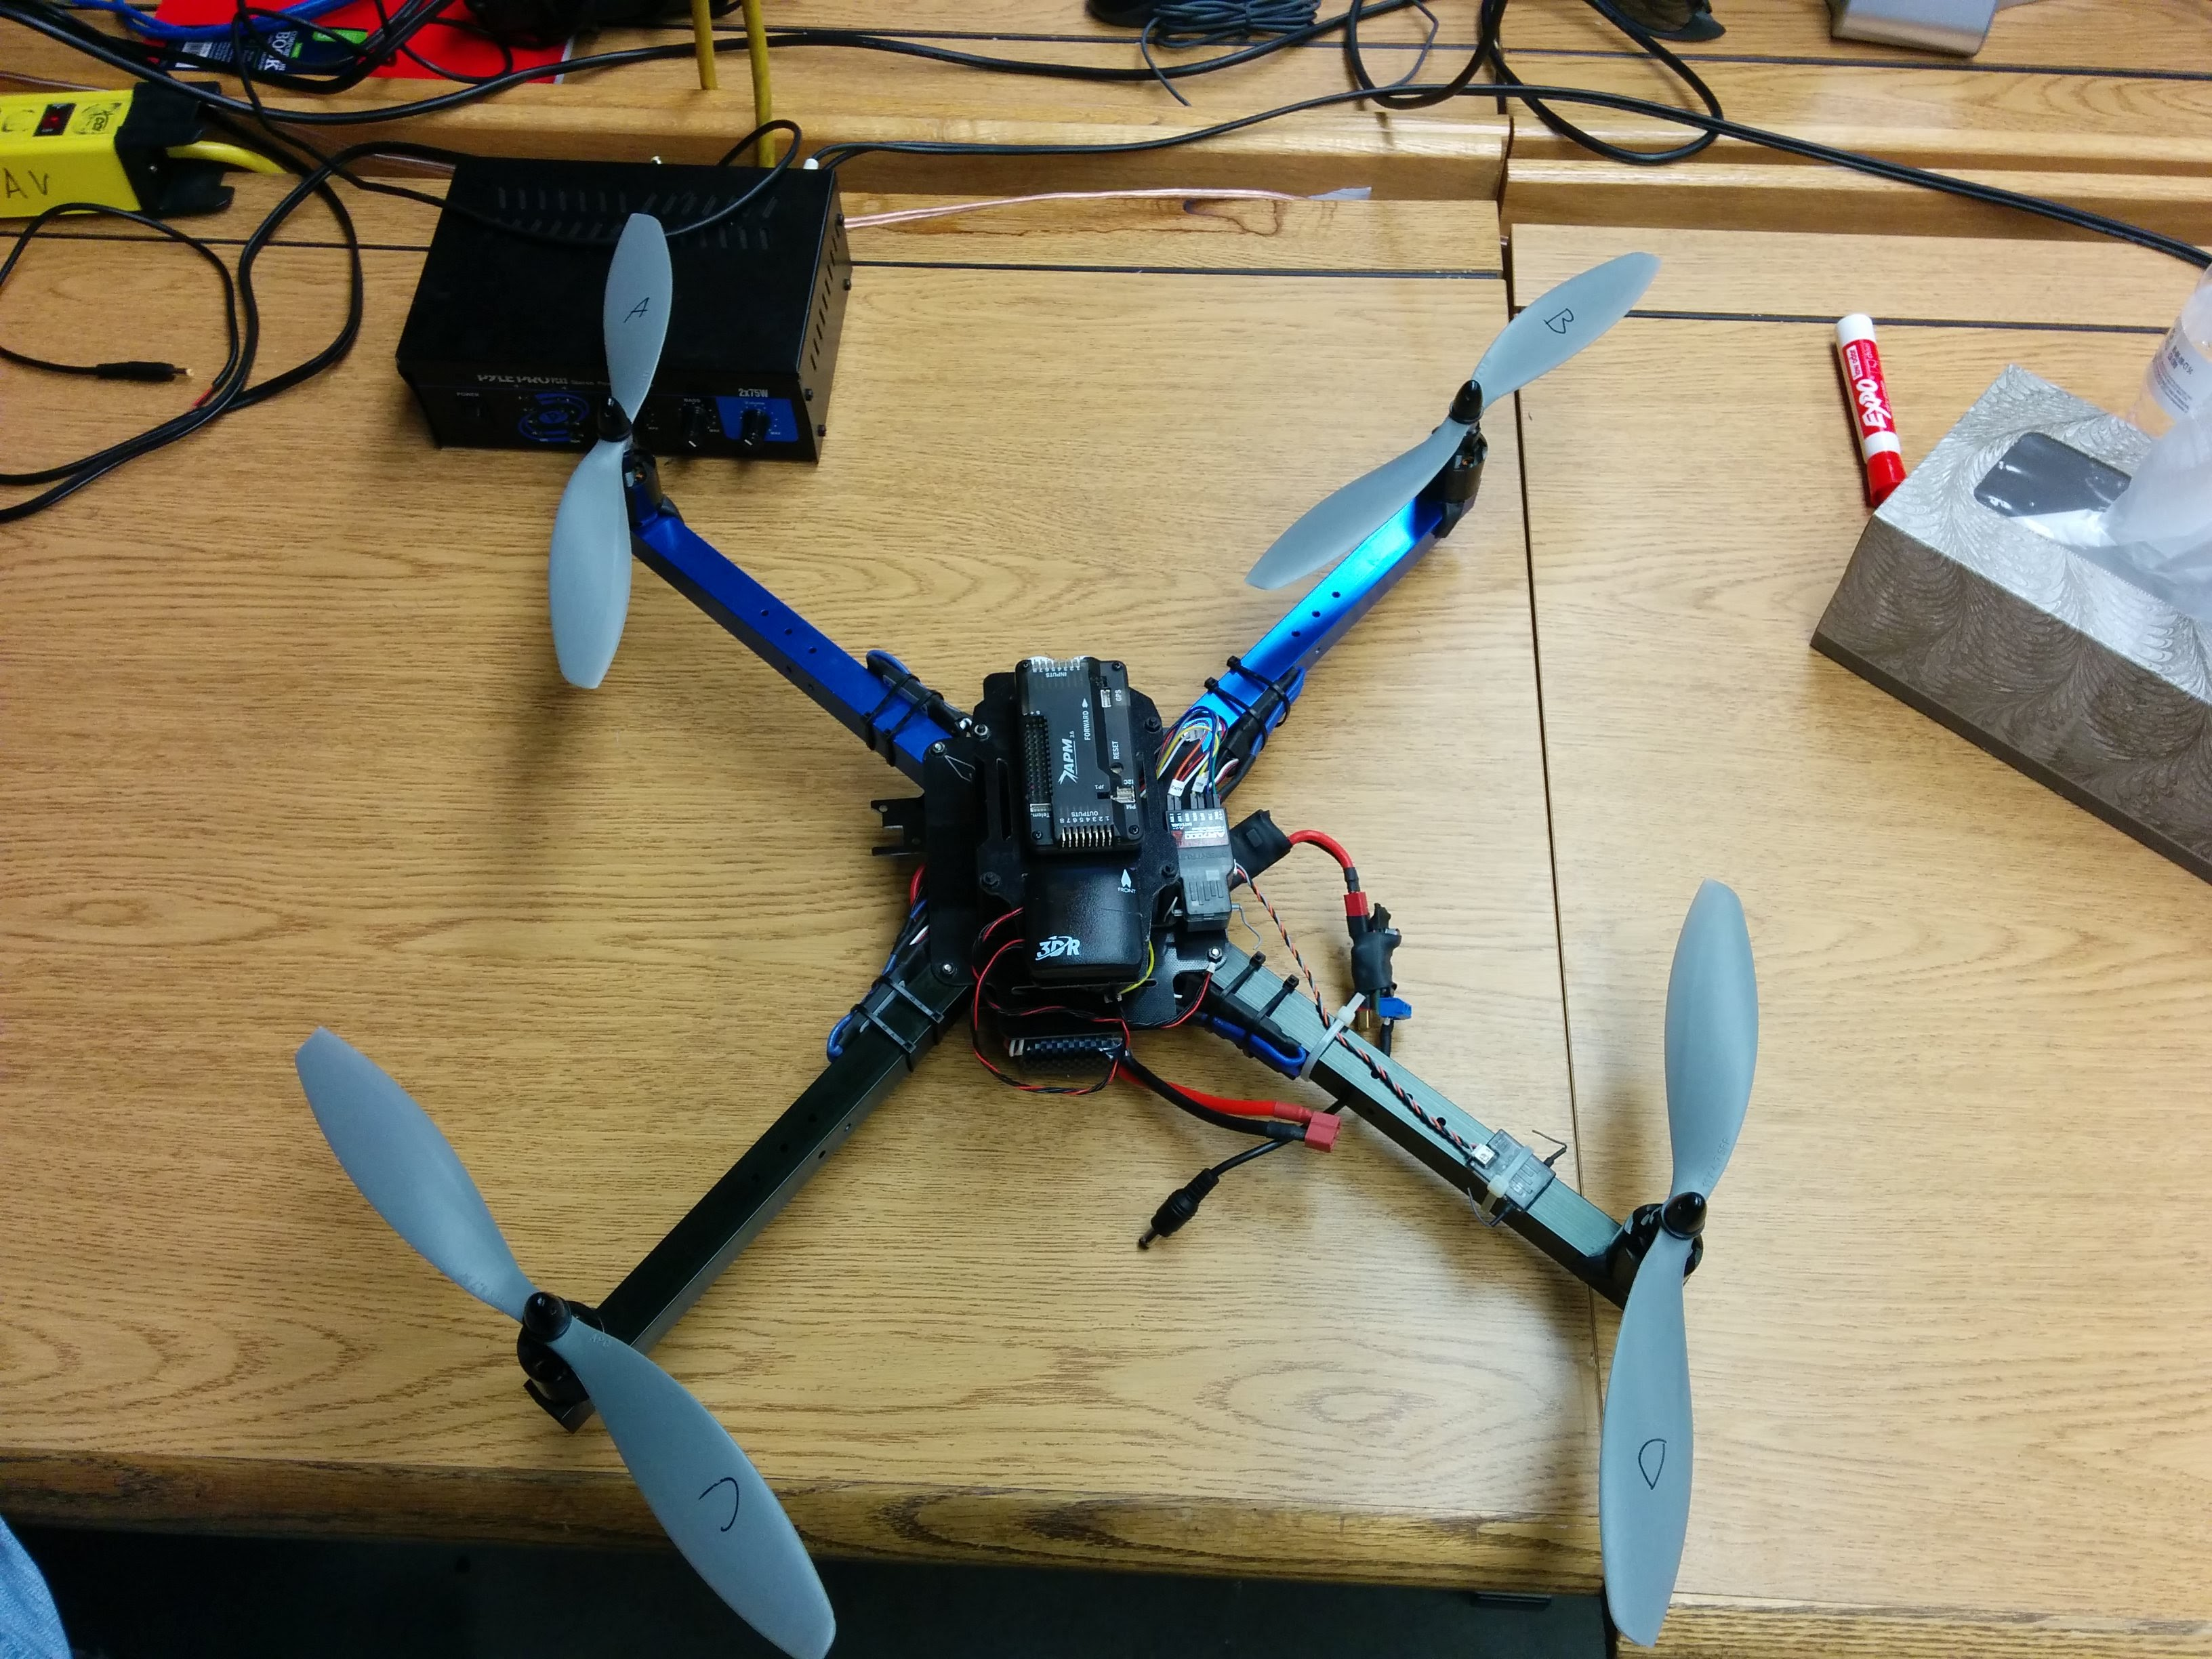
\includegraphics[width=0.4\textwidth]{images/quad}
\end{figure}

\end{frame}

\begin{frame}
\center \Large{{\textbf{Questions?}}}
\end{frame}

\end{document}
